\newif\ifpdf
\ifx\pdfoutput\undefined
  \pdffalse % we are not running PDFLaTeX
\else
  \pdfoutput=1 % we are running PDFLaTeX
  \pdftrue
\fi

\documentclass[letterpaper,oneside,12pt]{book}
\ifpdf
  \usepackage[pdftex]{graphicx}
  \pdfcompresslevel=9
\else
  \usepackage{graphicx}
\fi

\usepackage[american]{babel}
\selectlanguage{american}

% page layout
  \setlength{\hoffset}{-2.7cm} 
  \setlength{\voffset}{-.7in}
  \setlength{\textwidth}{15cm}
  \setlength{\oddsidemargin}{3.5cm}
  \setlength{\evensidemargin}{0.2cm}
  %\setlength{\topmargin}{2.5cm}
  \setlength{\headsep}{5ex}
\setlength{\textheight}{22cm}
  \renewcommand{\baselinestretch}{1.05}
\raggedbottom
  \newlength{\pictheight}
  \setlength{\pictheight}{\textheight}
  \addtolength{\pictheight}{-2cm}

%\newcommand{\todo}[1]{\textsf{\textbf{\Large{To do: #1}\normalsize}}}
\newcommand{\todo}[1]{}

% document
\begin{document}

\newcommand{\ie}{i.e.}
\newcommand{\eg}{e.g.}

\frontmatter
\begin{titlepage}
\hspace{-7mm}
\begin{minipage}{\textwidth}
\begin{center}
\vspace{.5cm}
{\huge \bf Software Design Document\\[1.5ex]}
{\large \bf for a specific implementation of `BCI2000'}
\\[1.5cm]
{\Large Gerwin Schalk\\}
{\Large Thilo Hinterberger\\}
{\Large Dennis J. McFarland\\[1.5cm]}
%
\begin{minipage}{13cm}
  \begin{minipage}[c]{13cm}
    \begin{center}
      {\Large \bf New York State Department of Health\\[2ex]}
      {\large \bf Wadsworth Center\\[0.5ex]
       Laboratory of Nervous Systems Disorders\\[4ex]}
      {\Large \bf Eberhard--Karls--Universit\"at T\"ubingen\\[2ex]}
      {\large \bf Medizinische Fakult\"at\\[0.5ex]
       Institut f\"ur Medizinische Psychologie\\[0.5ex]}
    \end{center}
  \end{minipage}
  \\[1.0cm]
  \begin{minipage}[c]{6cm}
    \centerline{
\includegraphics{figures/DOHlogo}}
  \end{minipage}
  \hspace{1.5cm}
  \begin{minipage}[c]{3cm}
    \centerline{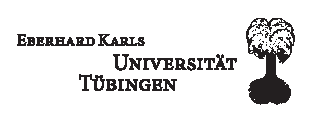
\includegraphics{figures/EKUlogo}}
  \end{minipage}
\end{minipage}
%
\\[0.5cm]
\textbf{Sponsors} \\
\textit{Jonathan R. Wolpaw and Niels Birbaumer}
\\[1.0cm]
{Albany, NY} \\[1ex]
{February 2000--May 2001}
\\[1ex]Updated May 2003, J\"urgen Mellinger
\end{center}
\end{minipage}
\end{titlepage}


\tableofcontents

\mainmatter

\chapter{Introduction}

\section{Involved Groups}

This document describes a project whose core contributors are the Brain-Computer 
Interface Research and Development Program at the Wadsworth Center of 
the New York State Department of Health and the Institute of Medical 
Psychology and Behavioral Neurobiology at the Eberhard-Karls-University in
T\"ubingen, Germany.

\section{Project Sponsors and Management}

The BCI2000 project is sponsored by Jonathan R. Wolpaw, MD and Prof. Dr. phil. 
Niels Birbaumer. The project is managed by Gerwin Schalk, MS.

\section{Acknowledgement}

We want to thank Dr. Thilo Hinterberger for his contributions during the initial 
phase of the project and Dr. Jouri Perelmouter for his input during the project 
design phase.


\chapter{Context and Purpose}

In recent years, many laboratories have begun to develop brain-computer 
interface (BCI) systems that provide communication and control capabilities to 
people with severe motor disabilities. Further progress and realization of 
practical applications depends on systematic evaluations and comparisons of 
different brain signals, recording methods, processing algorithms, output 
formats, and operating protocols.  However, the typical BCI system is designed 
specifically for one particular BCI method, and is therefore not suited to the 
systematic studies that are essential for continued progress. Furthermore, BCI 
design depends on the mastery of diverse areas such as computer science, 
neuroscience, physiology and psychology, and thus a tool that could facilitate 
the interaction and integration of competency in these areas would greatly 
foster the future development of BCI technology.

In response to this problem, we have developed and tested a general-purpose BCI 
research and development platform, called BCI2000. BCI2000 can incorporate alone 
or in combination any brain signals, signal processing methods, output devices, 
and operating protocols. To date, more than 25 laboratories around the world are 
using BCI2000 in a variety of studies. The BCI2000 system is available with 
free of charge for research or educational purposes at 
\texttt{http://www.bci2000.org}.

The background and rationale, as well as the general concept of BCI2000 is 
described in detail in a paper in \textit{IEEE Trans Biomed Eng} (Schalk et al., 
2004). This document goes beyond the scope of this article in that it defines 
the technical implementation-independent structures of BCI2000 (such as the 
communication protocol and the file format), i.e., in other words, the 
\emph{BCI2000 Standard}. This information is sufficient to create any addition 
to BCI2000 (in any language and on any operating system) that is compatible with 
this standard. BCI2000 is currently implemented using Borland C++ Builder on 
Windows platforms. For specific questions about these implementations 
(such as how to implement your own signal processing routines), please refer to 
the \emph{BCI2000 Software Design Document}.

\chapter{System Design} 

\section{Overview}

BCI2000 consists of four modules shown in Figure \ref{fig:modules} that 
communicate with each other. These modules are called \textit{Source}, 
\textit{Signal Processing}, \textit{Application}, and \textit{Operator}. We will 
refer to the three modules Source, Signal Processing and Application together as 
\textit{core modules}.


\begin{figure}[ht]
 \centerline{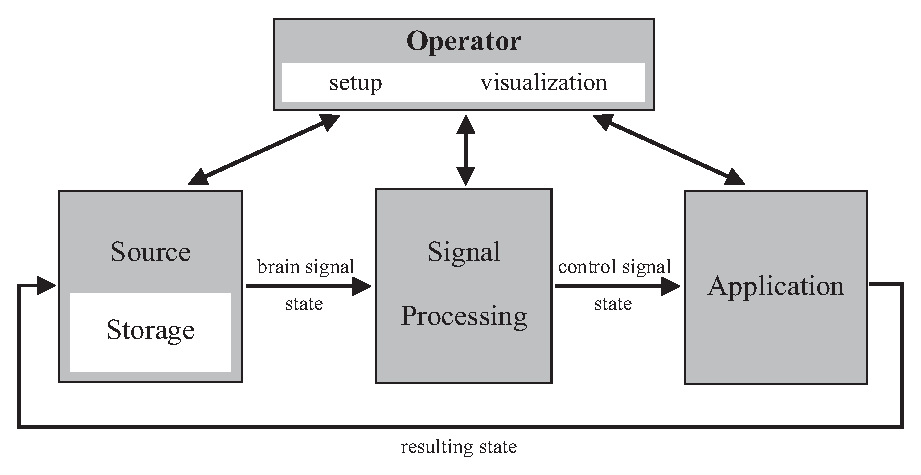
\includegraphics{figures/modules}}
 \caption{The functional modules and their interfaces}
 \label{fig:modules}
\end{figure}

%\section{Functional Modules}


\section{Core--Operator Communication}

\subsection{Introduction}

The same communication protocol is used between each of the three core modules 
and the operator module. Although it can be implemented on top of any transport 
protocol, it assumes the reliability of TCP (i.e., the protocol does not support 
acknowledgements or packet sorting or any other means of error correction).

Any message sent to or from any module is wrapped into packets as described in 
section \ref{protocol_definition}. This simple protocol allows for the delivery 
of data (e.g., parameters, visualization data, etc.), even if its content and 
nature are not known \textit{a priori}.


\subsection{Protocol Definition}
\label{protocol_definition}

Communication consists of messages that are sent and received asynchronously 
between any core module and the operator module. Each message starts with a one-
byte content descriptor and one-byte descriptor supplement, followed by a number that describes the length of the content.

\begin{figure}[ht]
 \centerline{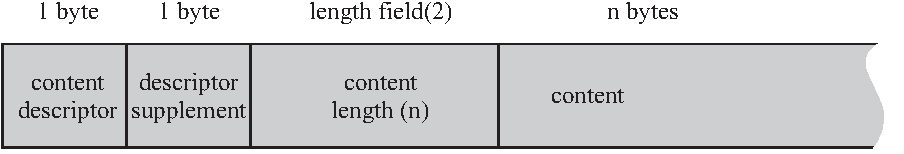
\includegraphics{figures/operator_prot}}
 \caption{Layout of one message in the protocol}
\end{figure}

The element denoted by ``length field(2)" was originally a two-byte integer 
field for the content length in little endian format. To allow for messages 
longer than 64k, we introduced a backwards-compatible extension: if the length 
is below 65535, it will still be transmitted as a two-byte integer in little 
endian format. Otherwise, the two bytes will contain the value 65535, and be 
followed by a decimal ASCII representation of the length, terminated with a zero 
byte. For other one- and two-byte length fields occurring in the protocol, the 
same scheme applies, generalized to be a ``length field(original number of 
bytes)" (Figure \ref{fig:length_field}).

\begin{figure}[ht]
 \centerline{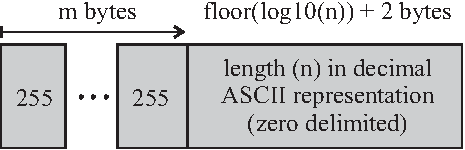
\includegraphics{figures/length_field}}
 \caption{Detailed layout of a length field(m) for a length $n \geq 2^m-1$}
 \label{fig:length_field}
\end{figure}

\begin{table}[ht]
 \centering
 \begin{tabular}{|l|l|}
  \hline
  \textbf{descriptor} & \textbf{description} \\
  \hline
  1 & status information string \\
  \hline
  2 & system parameter \\
  \hline
  3 & system state \\
  \hline
  4 & visualization data \\
  \hline
  5 & state vector \\
  \hline
  6 & system command \\
  \hline
 \end{tabular}
 \caption{The currently defined content descriptors}
\end{table}   


\subsection{Descriptor=1: Status Information Format}
\label{statusinfo_format}

This section describes the format of the message when the core message is 
a status information string (i.e., the message's descriptor is 1). In this 
case, the aforementioned content data is a line of ASCII characters 
in the following format:
\\[2ex]
\verb|xxx: status-line-text| 
\\[2ex]
xxx is a three digit number that describes the content of the status information string. 
The first digit is `1' for status information, `2' for successful operation, `3' 
for recoverable errors and `4' for fatal errors. The two remaining digits define 
the exact nature of the message, followed by a plain description.

This procedure is used to communicate errors and to convey status information (e.g.,
the operator module may display the remaining disc space on the Source module's
machine.)

\subsection{Descriptor=2: Parameter Format}
\label{parameter_format}

This section describes the format of the message when the core message is of 
type system parameter (i.e., the message's descriptor is 2). In this case, 
content data is a line of ASCII characters in the following format 
(Table \ref{tab:parametervariables} summarizes
the individual components in the parameter string):
\begin{verbatim}
Section DataType Name= Value DefaultValue LowRange HighRange
    // Comment CRLF
\end{verbatim}
If DataType is \textit{list, intlist} or \textit{floatlist}, the format is
as follows: 
\begin{verbatim}
Section DataType Name= (NumValues|Labels) Value(s) DefaultValue
    LowRange HighRange // Comment CRLF
\end{verbatim}
where \texttt{Labels} is a list of textual labels that optionally substitutes the number denoted by \texttt{NumValues}. A list of labels is enclosed by \verb|{}| or \verb|[]|, as in 
\verb|[low medium high]|.
\\[2ex]
If DataType is \textit{matrix}, the format is as follows:
\begin{verbatim}
Section DataType Name= (NumValuesDim1|LabelsDim1)
    (NumValuesDim2|LabelsDim2) Value(s) DefaultValue LowRange
    HighRange // Comment CRLF
\end{verbatim}
where again each NumValues entry may be substituted by a list of textual labels.

\paragraph{Special characters} To allow for special characters and white space 
within parameter values and textual labels, an URL-like encoding scheme is adopted.
In this encoding, a \texttt{\%} character followed by up to two hexadecimal digits 
represents a byte value in hexadecimal notation which is interpreted according to 
the ASCII-Latin1 character table.
Thus, \texttt{\%20} represents a space character, and \texttt{\%}, \texttt{\%0}, 
and \texttt{\%00} all represent an empty string value; \texttt{\%\%} represents the
\texttt{\%} character itself.
The line
\begin{verbatim}
Demo string SomeString= a%20string%20with%20spaces % % % 
    // White space example
\end{verbatim}
defines a parameter \textit{SomeString} which contains the value \textit{``a string
with spaces''}. The single \texttt{\%} characters indicate that the \textit{DefaultValue},
\textit{LowRange} and \textit{HighRange} fields should be empty strings.

\paragraph{Sub-parameters} Any parameter value may itself be a sub-parameter.
Sub-parameters are represented by a short-form
matrix definition omitting the \textit{Section} and \textit{Name} fields, enclosed in
a pair of braces:
\begin{verbatim}
Demo matrix NestedMatrices= 1 2 11 { matrix 2 2 1211 1212 1221 1222 } 
    // Nested matrix example
\end{verbatim}
will define a matrix parameter whose 1,2 entry is a 2x2 matrix.
While the syntax allows for any combination of parameter and subparameter types,
the current implementation of the parameter editor GUI does only support matrix-type
sub-parameters within matrices as in the example above.

\paragraph{Display Format} The comment line that is introduced by the two 
slashes (//) may contain a format identifier that is used by the Operator module
to modify the display of the particular parameter. Format identifiers are
strictly optional and are introduced as follows: \texttt{(identifier)}.
Currently, the following format identifiers are implemented:

\begin{table}[ht]
 \centering
 \begin{tabular}{|l|l|}
  \hline
  \textbf{Identifier} & \textbf{Description}\\
  \hline
  \texttt{(enumeration)} & a choice from an enumerated set of values \\
  \texttt{(boolean)} & a yes/no choice \\
  \texttt{(inputfile)} & path to a file to be opened for reading \\
  \texttt{(outputfile)} & path to a file to be opened for writing \\
  \texttt{(directory)} & path to a directory \\
  \texttt{(color)} & RGB color \\
  \hline
 \end{tabular}
 \caption{The currently defined format identifiers}
\end{table}   

\paragraph{\texttt{(enumeration)}}
The parameter value is presented as a drop down menu, with entries corresponding to the
possible values listed in the comment. The first part of the comment appears above
the drop down menu. All interpunction characters present in the comment are ignored.

The parameter's data type must be \texttt{int}.
All possible values must appear in the comment, and the parameter's LowRange and HighRange 
fields must be consistent with the enumeration. LowRange will usually be 0, but may be any
integer.
\begin{verbatim}
Breakfast int BreakfastDrink= 1 1 1 3
  // Drink for breakfast: 1 Tea, 2 Coffee, 3 Juice (enumeration)
\end{verbatim}
will display a drop down menu with entries ``Tea,'' ``Coffee,'', and ``Juice.''
The menu will be labeled ``Drink for breakfast.''

\paragraph{\texttt{(boolean)}}
The parameter value is presented as a check box; the first part of the comment appears
to the right of the check box. LowRange and HighRange must be 0 and 1.

The parameter's data type must be \texttt{int}.
To ensure human readability of parameter files, the possible values and their meaning may 
appear in the comment (e.\ g.\ \texttt{0:\ no, 1:\ yes}) but will not be displayed with the 
check box.
\begin{verbatim}
Breakfast int ServeBreakfast= 1 1 0 1
  // Serve breakfast: 0 no, 1 yes (boolean)
\end{verbatim}
will display a check box labeled ``Serve breakfast.''

\paragraph{\texttt{(inputfile)(outputfile)(directory)}}
The parameter value is presented as an edit field. Beside the edit field, a button
exists that opens up a file or directory choosing dialog when clicked.

The parameter's data type must be \texttt{string}.
\begin{verbatim}
Breakfast string WakeupSound= doorbell.wav % % %
  // Sound to play in the morning (inputfile)
\end{verbatim}

\paragraph{\texttt{(color)}}
The parameter value is presented as an edit field. Right to the edit field, a button
exists that opens up a color chooser dialog when clicked.

The parameter's data type must be \texttt{string}, with its value containing the color
in hexadecimal RGB encoding:
\begin{verbatim}
Breakfast string TableClothColor= 0x00FF00 0xFFFFFF 0x000000 0xFFFFFF
  // Color of table cloth to put up for breakfast (color)
\end{verbatim}

\paragraph{Grouping Parameters}
A user interface may use parameters' \texttt{Section} fields to collect parameters into
groups, \eg{} by displaying all parameters with identical section fields on the same
register tab of a GUI parameter editor dialog window.

In the \texttt{Section} field, finer grained grouping may be expressed by specifying
sub-sections separated by colon characters, \eg{} a \texttt{Section} value of
\verb|UsrTask:WindowDimensions|
will indicate that a parameter belongs to a \texttt{WindowDimensions} subsection of
a section called \texttt{UsrTask}. A parameter editor implementation might 
choose to display the respective parameter on a register tab called ``UsrTask'' and
inside a group box labelled ``WindowDimensions''.

Although any number of sub-sections may be present in the \texttt{Section} field, 
a user interface implementation may ignore sub-section entries below a 
level chosen by the implementer.

\subsubsection{}
The parameter format does not only apply to the interaction between core and 
operator, but also reflects the data format of BCI2000 parameter files (i.e., 
files with extension .prm) as well as the parameter portion of the BCI2000 data 
files (i.e., files with extension .dat) files. The core modules and the operator 
module also use this format to communicate in the system initialization phase 
(as described in section \ref{system_init}).

\begin{table}[ht]
 \centering
 \begin{tabular}{|l|l|}
  \hline
  Section \\
  \hline
  Type \\
  \hline
  \textbf{Name} \\
  \hline
  ${\left[
    \mbox{(NumValuesDim1$\mid$\{ LabelDim1.1 LabelDim1.2 ... \})}
    \atop
    \mbox{[(NumValuesDim2$\mid$\{ LabelDim2.1 LabelDim2.2 ... \})]}
    \right]}$ \\
  \hline
  Value(s) \\
  \hline
  DefaultValue \\
  \hline
  LowRange \\
  \hline
  HighRange \\
  \hline
  Comment incl. format identifiers \\
  \hline
 \end{tabular}
 \caption{Definition of variables in the parameter string}
 \label{tab:parametervariables}
\end{table}   

For data types \textit{list, intlist} and \textit{floatlist}, \textit{NumValues} 
indicates how many values are following. The separate values are then 
delimited by white spaces. In case of data type \textit{matrix}, the transmitted 
values represent the matrix as follows: the first NumValuesDim2 values are 
value(0, t), followed by NumValuesDim2 values value(1, t), etc.; in case that 
labels are specified in place of value counts, the analogy holds with the value 
counts given by the number of labels for the dimension in question.\\

Each core module knows the data types of the parameters it is requesting and 
thus does not need a parameter data type definition. However, the operator 
module uses the data type definitions as listed in table 
\ref{tab:parametervariables} to create their graphical representation. Section 
\ref{system_params} describes a list of pre-defined system parameters.

\todo{Describe proposal for parameter data type for state definition, e.g.,
TargetCode 1 Feedback 1}

\subsection{Descriptor=3: State Format}
\label{state_format}

This section describes the format of the message when the core message is of 
type system state (i.e., the message's descriptor is 3). In this case, the 
aforementioned content data is a line of ASCII characters (parameters
delimited by spaces) in the following format:
\\[2ex]
\verb|Name Length Value ByteLocation BitLocation CRLF|
\\[2ex]
with BitLocation ranging from 0..7.
The core modules and the operator module use this format to communicate in 
the system initialization phase (as described in section \ref{system_init}), 
as well as during system performance (section \ref{system_performance}) and 
for system termination (section \ref{system_termination}). Table 
\ref{state_table} defines the maximum length for each parameter.

\begin{table}[ht]
 \centering
 \begin{tabular}{|l|l|}
  \hline
  \textbf{Name} & \textbf{Max. Length} \\
  \hline
  Name & 30 \\
  \hline
  Length & 2 \\
  \hline
  Value & 5 \\
  \hline
  ByteLocation & 1 \\
  \hline
  BitLocation & 1 \\
  \hline
 \end{tabular}
 \caption{Definition for variables in the state string}
 \label{state_table}
\end{table}   

\subsection{Descriptor=4: Visualization Data Format}
\label{visualizationdata_format}

This section describes the format of the message when the core message is of 
type visualization data (i.e., the message's descriptor is 4). In this case (see 
figure \ref{visualizationprotocol}), the content descriptor describes the 
requested visualization type. The only currently defined types are 1 (a graph of 
\textit{n} channels and \textit{m} samples), 2 (a text memo), and 255 
(visualization configuration).

\begin{figure}[ht]
 \centerline{\scalebox{0.75}{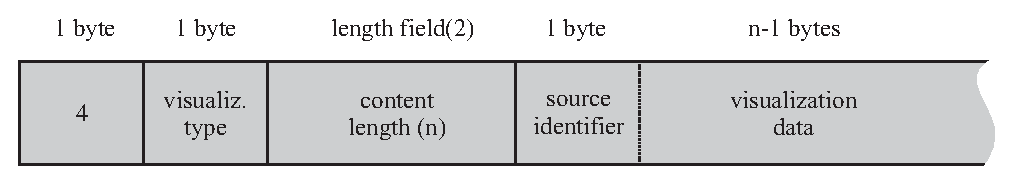
\includegraphics{figures/operator_prot_visualization}}}
 \caption{One message in the protocol if it is of type "visualization data"}
 \label{visualizationprotocol}
\end{figure}

\begin{figure}[ht]
 \centerline{\scalebox{0.75}{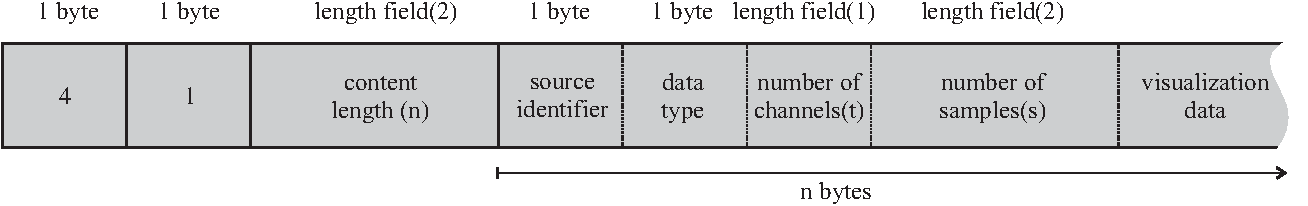
\includegraphics{figures/operator_prot_visualization_type1}}}
 \caption{One message if visualization type is 1 (i.e., a graph)}
 \label{visualizationprotocol_type1}
\end{figure}

Figure \ref{visualizationprotocol_type1} illustrates the protocol when the 
visualization type is 1. The source identifier defines a unique number 
identifying the process/filter that generated the data. The data type can be 
\begin{itemize}
\item 0 \texttt{(SignalType::int16)} for integers in little endian format.
\item 1 \texttt{(SignalType::float24)} for 3-byte floating-point values:
The first two bytes (i.e., A) define 
the mantissa (signed two-byte integers in little endian format) and the third 
byte (i.e., B) defines the exponent (signed one-byte integer). The actual floating 
point value is then calculated as follows: $value=A*10^{B}$.
\item 2 \texttt{(SignalType::float32)} for 4-byte floating-point values in IEEE 754 format transmitted in little endian byte order.
\item 3 \texttt{(SignalType::int32)} for 4-byte signed integer values transmitted in little endian byte order.
\end{itemize}

The number of channels and samples are self explanatory.
Figure \ref{visualization_type1} illustrates how the data is transferred.

\begin{figure}[ht]
 \centerline{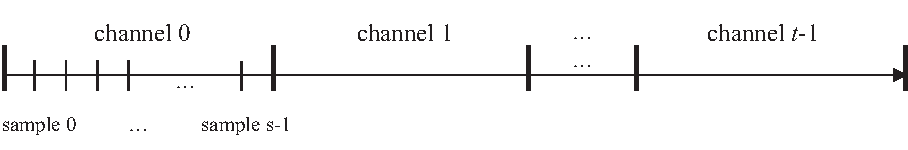
\includegraphics{figures/visualization_type1}}
 \caption{Graphical representation of the transmitted visualization data format}
 \label{visualization_type1}
\end{figure}

\begin{figure}[ht]
 \centerline{\scalebox{0.75}{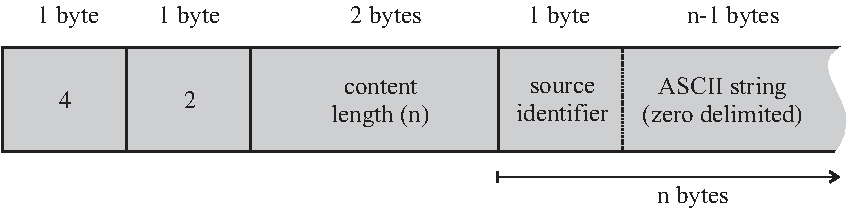
\includegraphics{figures/operator_prot_visualization_type2}}}
 \caption{One message if visualization type is 2 (i.e., a text memo)}
 \label{visualizationprotocol_type2}
\end{figure}

Figure \ref{visualizationprotocol_type2} illustrates the protocol when the 
visualization type is 2. The source identifier is a number uniquely 
identifying the process/filter that generated the data. The following ASCII
text is zero delimited.

\begin{figure}[ht]
 \centerline{\scalebox{0.75}{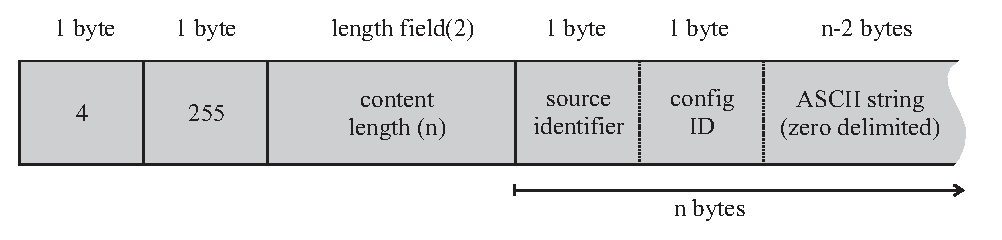
\includegraphics{figures/operator_prot_visualization_type255}}}
 \caption{One message if visualization type is 255 (i.e., visualization configuration)}
 \label{visualizationprotocol_type255}
\end{figure}

Figure \ref{visualizationprotocol_type255} illustrates the protocol when the 
visualization type is 255. The source identifier is a number 
identifying the process/filter that generated the data. The different 
configuration IDs are described in Table \ref{tab:viscfg_table}.

\begin{table}[ht]
 \centering
 \begin{tabular}{|l|l|}
  \hline
  \textbf{Cfg ID} & \textbf{Description} \\
  \hline
  1 & Window Title \\
  \hline
  2 & Minimum Value \\
  \hline
  3 & Maximum Value \\
  \hline
  4 & Number of Samples \\
  \hline
  5 & X Axis Label \\
  \hline
  6 & Y Axis Label \\
  \hline
  7 & Number of Subsequent Channels displayed on the same base line \\
  \hline
  8 & Graph Type (Polyline or 2D Field) \\
  \hline
  9 & Polyline Graph Type \\
  \hline
  10 & Show Base Lines (1 or 0) \\
  \hline
  11 & List of Channel Colors \\
  \hline
  12 & 2D Field Graph Type \\
  \hline
  13 & Unit for Sample dimension \\
  \hline
  14 & Unit for Channel dimension \\
  \hline
  15 & Unit for Values \\
  \hline
  16 & Number of Lines for a Memo \\
  \hline
 \end{tabular}
 \caption{The various IDs for visualization configuration}
 \label{tab:viscfg_table}
\end{table} 

The ASCII string then contains the configuration option, as defined by the 
configuration ID. For example, it might contain "128" if the configuration ID 
is 4. This will configure the graph to contain exactly 128 samples. When the 
configuration ID is 5 or 6 (axis labels), the ASCII string consists of a sample 
number (three digits), a space, and the axis label. Thus, one message configures 
exactly one axis label. As an example and for an X-axis label, the string "003 
4.75 Hz" would result in a graph, in which the third sample is labeled "4.75 
Hz."


\subsection{Descriptor=5: State Vector}
\label{statevector}

This section describes the format of the message when the core message is of 
type state vector (i.e., the message's descriptor is 5). 

The state vector is defined by a series of \textit{StateVectorLength} subsequent 
bytes. The structure of these bytes is defined in \ref{statevector_format}.


\subsection{Descriptor=6: System Command}
\label{sec:syscmd}

This section describes the format of the message when the core message is of 
type system command (i.e., the message's descriptor is 6). 

The system command consists of an ASCII string that may end with a zero byte 
(i.e., ASCII code 0).

The nature of these system commands is defined by the specific implementation of 
the modules.


\section{Inter--Core Communication}

\subsection{Introduction}

Unlike the bidirectional communication between core modules and the operator 
module, communication within the core modules is unidirectional. The initial 
setup determines the exact nature of this communication and data is transmitted 
with the same protocol as described in Section \ref{protocol_definition}. The 
following sections describe the transferred brain signal, state vector, and 
control signal. The state vector is always transmitted before the brain 
signal or control signal. Whenever \textit{Running} switches from 0 to 1, the 
system is re-initialized.

\subsection{Brain Signal Format}
\label{sec:eegsigformat}

The brain signal is transmitted similarly to visualization data (i.e., as 
described in Section \ref{visualizationdata_format}). The visualization type is 
set to 1 (i.e., graph), source identifier is set to 0. Data type, channels and samples reflect the actual format of data transmitted.


\subsection{State Vector Format}
\label{statevector_format}

The state vector is transferred as type state vector (see Section 
\ref{statevector}). The content descriptor is 5 and the descriptor supplement is 
undefined. Its content consists of a series of \textit{StateVectorLength} bytes. 
The value of a given state within the state vector is determined by its byte/bit 
location and length definition. The bits in the state vector are always sorted 
in ascending order, e.g., for a state with a length of 7 bits, starting at byte 
location 2, bit location 3, bit zero is first (byte 2, bit 3), and the highest 
bit (bit 7) is last (byte 3, bit 1).

\subsection{Control Signal Format}

Control signals are transmitted similarly to the Brain Signal (see Section 
\ref{sec:eegsigformat}) with \textit{NumControlSignals} channels and one sample 
per channel.


\section{System-Wide Parameters}
\label{system_params}

\subsection{Introduction}

System--wide parameters are published and initialized during system--startup, as 
described in section \ref{system_init}. Each parameter is described by the 
section it belongs to, a data type descriptor, its name, value(s), default 
value, and a range of valid numbers. Parameter names are unique across the 
entire system.

\subsection{Defined Data Types}

\vspace{.5cm}

\begin{flushleft}

\begin{centering}
 \begin{tabular}{|l|l|}
  \hline
  \textbf{Data Type} & \textbf{Description} \\
  \hline
  char & one character \\
  \hline
  string & a string of characters \\
  \hline
  int & a 16-bit signed integer \\
  \hline
  longint & a 32-bit signed integer \\
  \hline
  float & a single-precision floating point \\
  \hline
  bool & a boolean value (0..false, 1..true) \\
  \hline
  list & a list of untyped values \\
  \hline
  intlist & a list of 16-bit signed integers \\
  \hline
  floatlist & a list of single-precision floating points \\
  \hline
  matrix & a matrix of untyped values \\
  \hline
 \end{tabular}
% \caption{Data type definition for variables in the parameter string}
\end{centering}   

\vspace{.5cm}

\newpage

\subsection{Defined Sections and Parameter Names}

Section names can be defined by the parameter definition. The only reserved 
section name is \emph{System}. User-defined parameters may not go into this 
section.

The BCI2000 standard requires the definition of the following parameters:

\raggedright \large Section ``Source" \normalsize
\\[2ex]
%\begin{displaymath}
 \begin{tabular}{|l|l|l|}
  \hline
  \textbf{Type} & \textbf{Parameter Name} & \textbf{Description}\\
  \hline
  int & SoftwareCh & number of digitized and stored channels \\
  \hline
  int & SampleBlockSize & number of transmitted samples \\
  \hline
  intlist & TransmitChList & list of channels to transmit \\
  \hline
  int & SamplingRate & data acquisition's sampling rate in Hz \\
  \hline
 \end{tabular}
 %\caption{Parameter names in section Source}
%\end{displaymath}

\vspace{.5cm}
\raggedright \large Section ``Storage" \normalsize
\\[2ex]
%\begin{displaymath}
 \begin{tabular}{|l|l|l|}
  \hline
  \textbf{Type} & \textbf{Parameter Name} & \textbf{Description}\\
  \hline
  string & SubjectName & subject alias \\
  \hline
  string & SubjectSession & session number (max. 3 characters) \\
  \hline
  string & SubjectRun & digit run number (max. 3 characters) \\
  \hline
  string & FileInitials & top level directory for saved files \\
  \hline
 \end{tabular}
% \caption{Parameter names in section Storage}
%\end{displaymath}

\vspace{.5cm}

\newpage

\large Section ``Filtering" \normalsize \\[1ex]

%\begin{table}[!ht]
 \begin{tabular}{|l|l|l|}
  \hline
  \textbf{Type} & \textbf{Parameter Name} & \textbf{Description}\\
  \hline
  int & NumControlSignals & number of transmitted control signals \\
  \hline
  int & AlignChannels & whether or not to align channels in time \\
  \hline
  floatlist & SourceChOffset & offset in A/D units\\
  \hline
  floatlist & SourceChGain & factor to convert A/D units to $\mu$V \\
  \hline
  floatlist & SourceChTimeOffset & offset of sample at each channel in time (from 0..1) \\
  \hline
 \end{tabular}
% \caption{Parameter names in section Filtering}
%\end{table}   

%\vspace{.5cm}
%\large Section "Visualization" \normalsize \\[1ex]

%\begin{table}[!ht]
% \begin{tabular}{|l|l|l|}
%  \hline
%  \textbf{Type} & \textbf{Parameter Name}\\
%  \hline
%  int & ViewSourceCh[SoftwareCh, ViewSourceBlockSize]\\  
%  \hline
%  int & ViewTransmitCh[TransmitCh, ViewTransmitBlockSize]\\
%  \hline
%  int & ViewControlCh [ControlCh, ViewControlBlockSize] \\
%  \hline
%  float & ViewFFTCh[FFTCh, ViewFFTBlockSize] \\
%  \hline
%  float	& ViewSWCh[SWCh, ViewSWBlockSize] \\
%  \hline
% \end{tabular}
% \caption{Parameter names in section Visualization}
%\end{table}   

\vspace{.5cm}
\large Section ``System" \normalsize \\[1ex]

%\begin{table}[!ht]
 \begin{tabular}{|l|l|l|}
  \hline
  \textbf{Type} & \textbf{Parameter Name} & \textbf{Description}\\
  \hline
  string & EEGsourceIP & IP address the Source module listens on\\  
  \hline
  int & EEGsourcePort & port the Source module listens on\\  
  \hline
  string & SignalProcessingIP & IP address Signal Processing listens on\\  
  \hline
  int & SignalProcessingPort & port Signal Processing listens on\\  
  \hline
  string & ApplicationIP & IP address the Application module listens on\\  
  \hline
  int & ApplicationPort & port the Application module listens on\\  
  \hline
  int & StateVectorLength & the length of the state vector in bytes\\  
  \hline
 \end{tabular}
% \caption{Parameter names in section System}
%\end{table}   

\end{flushleft}


\section{System-Wide States}
\label{states}

\subsection{Introduction}

While the purpose of system-wide parameters is to define the static 
configuration, the state information provides dynamic information about the 
current state of the system, e.g., whether the system is running or not.

States are published and initialized during system-startup, as described in 
section \ref{system_init}. A state is described by its name, its length (in 
bits) and its location (defined by start byte and bit in the state vector). 
The state vector is always transferred as a full number of bytes (specifically, 
\textit{StateVectorLength} bytes) (i.e., the end is padded with zeroed 
bits if necessary).

\subsection{The State Vector}

While the operator module constructs the state vector after receiving 
all requests for states from the core modules, some states do not need to be
to be requested -- they are created automatically. They are:
\\[2ex]
\begin{tabular}{|l|l|l|}
 \hline
 \textbf{Length} & \textbf{Name} & \textbf{Description}\\
 \hline
 16 & SourceTime & 16-bit unsigned integer; resolution 1 ms \\  
 \hline
 16 & StimulusTime & 16-bit unsigned integer; resolution 1 ms \\  
 \hline
 1 & Running & 1: system is running, 0: system is suspended\\  
 \hline
\end{tabular}


\section{System Initialization}
\label{system_init}

\subsection{Introduction}

This section describes the system initialization process. Since the system is a 
distributed system of encapsulated modules, this procedure ensures a proper and 
well defined information flow at start-up.

\subsection{Startup Sequence}

The operator module must be started first. Since in most cases the IP address of 
the operator module can be more easily statically defined, its IP address and 
port number(s) have to be provided to the core modules. It listens on ports 4000 
(for Source), 4001 (for Signal Processing), and 4002 (for Application) and 
waits for the respective core module to connect. Each can connect to its 
assigned port on the operator module in any order. Upon start--up, each core 
module opens a listening socket on an arbitrary port number.

\subsection{Publishing Phase}

Upon connection, each core module publishes its parameters to the operator 
module, as described in section \ref{parameter_format}. After publishing its 
parameters, each core module publishes the states it requests, as described in 
chapter \ref{state_format}. At this time, the operator module ignores every 
field except \textit{Name} and \textit{Length}, which it needs to construct the 
state vector.

For this and all subsequent communication, the modules use the protocol 
described in chapter \ref{protocol_definition}. Following the last state, each core module sends a system command containing the string \texttt{EndOfState}.
On receiving this command from all core modules, the operator module ends 
this initial publishing phase.

\subsection{Information Phase}

The operator module processes the received parameters and states. It creates a 
list of all parameters and all states and creates the state vector (double 
parameters or states are ignored). At this point, the operator module may modify 
the value of the parameters and states (depending on the investigator's input or 
the parameter file). The operator module then uses the same channel on which it 
received data from the core modules to send back to all core modules a list of 
all system-wide parameters and system-wide states (in any order). Since the IP 
address and port number on which the core modules listen for data from other 
core modules are published in system parameters as described, each module now 
knows where to send its data. The connections from the core modules to the 
operator module remain open (all subsequent traffic will go through these 
connections).

As in the publishing phase, the Information Phase ends when a system command 
\texttt{EndOfState} is sent.

In order to maintain integrity throughout operation, no parameters or states 
should be added to or removed from the system beyond this point.

\subsection{Preflight Phase}

Each core module declares whether it can process data with the received
parameters and states, or indicates errors by sending descriptions into
an error channel. If any errors are indicated during the preflight phase,
the module will not initiate the initialization phase; the operator module
will display the errors, prompting the user to fix the problems detected, 
and not offer the ``Start" option.

\subsection{Initialization Phase}

Each core module uses the information in the received parameters to configure and 
initialize its operation. It also opens an active (i.e., client) connection 
to the other core module it must connect to, i.e., Source opens a 
connection to Signal Processing, Signal Processing to Application and 
Application to Source.

Each core module sends a status message (see \ref{statusinfo_format}) to the 
operator that indicates either successful or failed initialization. The 
Initialization Phase ends when all core modules indicate successful 
configuration.


\section{System is Running}
\label{system_performance}

At the end of the Initialization Phase, the system is fully configured. All 
parameters and states (and positions thereof in the state vector) are defined. 
During system operation, the Operator module must send states only to the Source 
module and Signal Processing and Application must disregard any state that the 
Operator does send to them. 

The system is started when the Operator module sets the state \textit{Running} 
to 1 and sends it to the Source module. 


\section{System is Suspended}
\label{sec:system_suspended}

The system is suspended when \textit{Running} is 0. Any module shall disregard a 
change in parameters if the system is not suspended. Data flows through the 
system and it is up to each module to decide how to process these data. The 
Application, for example, might give visual feedback that indicates that the 
system is suspended. As long as operation is suspended (i.e., \textit{Running} 
is 0), any module might update system parameters and send them back to the 
Operator.


\section{System Termination}
\label{system_termination}

If any module detects a dropped connection to the Operator, it must shut down 
all other socket connections and terminate.

\section{File Formats}

\subsection{Data File}

The data file consists of a header and the actual raw brain signals. The header 
consists of a definition of all system parameters and states. Thus, parameters 
must not change within one data file.

\subsubsection{Header}

The header of a data file consists of lines of ASCII characters. Its total 
length is determined by the parameter HeaderLen in the first line.
The first line specifies general parameters, while the following define all
states in the state vector, as well as all the current parameters.
The number of bytes in the state vector is determined by the sum of the
lengths (defined in bits) for all states, rounded up to the next byte
(which equals the value of \textit{StateVectorLength} in both the first 
line and, since \textit{StateVectorLength} is also a system-wide parameter,
in one of the lines in the \texttt{[Parameter Definition]} section).
Thus, the data file can be read (although not fully interpreted) by reading
the first line.
The state definitions have the same format as described in \ref{state_format}
(although their values in the header are irrelevant, since they are defined
for each sample in the data file).
The parameter definitions have the format described in section
\ref{parameter_format}.
Since version 1.1, the first line begins with a \textit{BCI2000V} field
containing a version number in floating-point format, and ends with a 
\textit{DataFormat} field describing the format of the binary data as
\textit{int16}, \textit{int32}, or \textit{float32}.
A missing \textit{BCI2000V} field indicates a file format version of 1.0, 
and a \textit{DataFormat} of \textit{int16}.

\begin{flushleft}
\begin{footnotesize}
\begin{verbatim}
BCI2000V= 1.1 HeaderLen= l SourceCh= m StateVectorLength= k DataFormat= f CRLF
[ State Vector Definition ] CRLF
Name1 Length1 Value1 ByteLocation1 BitLocation1 CRLF
Name2 Length2 Value2 ByteLocation2 BitLocation2 CRLF
Name3 Length3 Value3 ByteLocation3 BitLocation3 CRLF
...
[ Parameter Definition ] CRLF
Section1 DataType1 Name1= Value1 DefaultValue1 LowRange1 HighRange1 // Comment CRLF
Section2 DataType2 Name2= Value2 DefaultValue2 LowRange2 HighRange2 // Comment CRLF
Section3 DataType3 Name3= Value3 DefaultValue3 LowRange3 HighRange3 // Comment CRLF
...
CRLF
\end{verbatim}
\end{footnotesize}
\end{flushleft}
The binary data directly follows this last CRLF.

\subsubsection{Binary Data}
\label{binary_data}

For each sample, data values for all channels are stored, followed by \textit{StateVectorLength} bytes for the state vector.
Data samples are stored in little endian format depending on the \textit{DataFormat} field:
\begin{center}
 \begin{tabular}{|l|l|}\hline
  \textbf{DataFormat field} & \textbf{data type} \\ \hline 
  int16 & 2-byte signed integer \\
  int32 & 4-byte signed integer \\
  float32 & 4-byte floating point (IEEE 754) \\ \hline 
 \end{tabular}\\
\end{center}
The number of samples in the file can be calculated as follows: 
$$
  \textrm{samples}
    =\frac{(\textrm{file size in bytes})-\textrm{HeaderLen}}
    {\textrm{(data value size in bytes)}\times\textrm{SourceCh}+\textrm{StateVectorLength}}
$$

\subsection{Parameter File}

A parameter file consists of lines of ASCII in the same format as the parameter section in the data file header and as described in section \ref{parameter_format}.

\newpage
\subsection{BCI2000 File Extensions}

The following table lists all extensions for BCI2000 data files:
\vspace{0.5cm}\\
\begin{centering}
 \centering
 \begin{tabular}{|l|l|}
  \hline
  \textbf{description} & \textbf{extension} \\
  \hline
  Data file & .dat \\
  \hline
  Parameter file & .prm \\
  \hline
  Application log file & .apl or .log \\
  \hline
  Statistics log file & .sta \\
  \hline
 \end{tabular}
 %\caption{Reserved extensions for BCI2000 data files}
\end{centering}   

\section{Glossary} 

\textbf{little endian} \\
In little endian, the binary representation of a 16-bit integer is: low-byte (bits 0-7)
first, followed by the high-byte (bits 8-15).
\\[2ex]
\textbf{CR} \\
stands for carriage return, or {ASCII} code 10.
\\[2ex]
\textbf{LF} \\
stands for line feed, or {ASCII} code 13.
\\[2ex]
\textbf{CRLF} \\
stands for carriage return and line feed, or (subsequent) {ASCII} codes 10 and 13.
\\[2ex]
\textbf{parameter} \\
A parameter is a static and global variable that describes some aspect of the 
system configuration. Parameters can only be created during the system startup phase, and changed during the information phase or when the system is in suspended state.
\\[2ex]
\textbf{state} \\
A state is a n-bit value that describes some aspect of the current system 
status. In communication, a state is represented as described in section
\ref{state_format}.
\\[2ex]
\textbf{state vector} \\
The state vector holds all values for all states that are packed together in one
array of bytes of length \textit{StateVectorLength}.


\backmatter
\end{document}

